\section{Versuch 1 - Ausgleichspolynom der Beschleunigungssensoren}
Das Ziel des ersten Versuchs ist ein Ausgleichspolynom zu ermitteln um die Rohwerte der Sensoren in SI-Einheiten umzurechnen. Die Sensoren geben für jede Beschleunigungsachse 16-Bit Werte aus, welche im Zweierkomplement dargestellt werden. In dem Versuch wird die Würfelseite in sieben verschiedenen Positionen ($\varphi \in \{-45^{\circ}, -30^{\circ}, -15^{\circ}, 0^{\circ}, 15^{\circ}, 30^{\circ}, 45^{\circ} \} $) fixiert und jeweils $m = 1000$ Beschleunigungswerte in X- und Y-Richtung aufgenommen. Da die Würfelseite in den Positionen stillsteht ist der Sollwert der Beschleunigungssensoren bekannt. Folglich kann ein Polynom ersten Grades approximiert werden um die Mittelwerte der Rohdaten in die entsprechenden Mittelwerte umzurechnen.

\subsection{Rohwerte}
Die folgenden Abbildungen zeigen die Rohwerte der beiden Sensoren in X- und Y-Richtung in den verschiedenen Positionen.

\subsubsection{Rohwerte bei $\varphi = -45^{\circ}$}
\begin{figure}[h]
	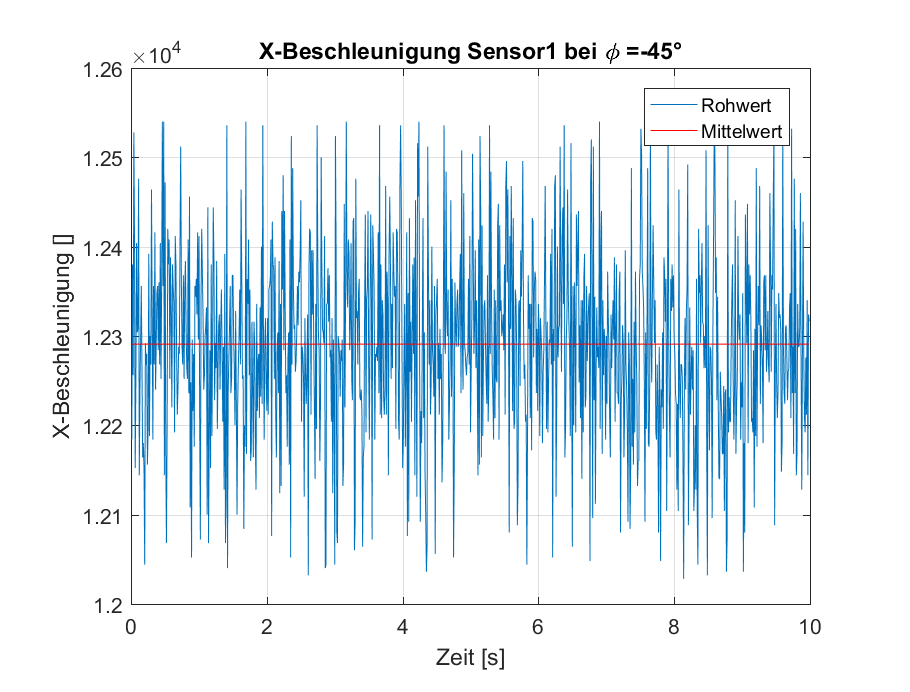
\includegraphics[width=0.5\linewidth]{img/X1__dd___phi_-45.eps}
	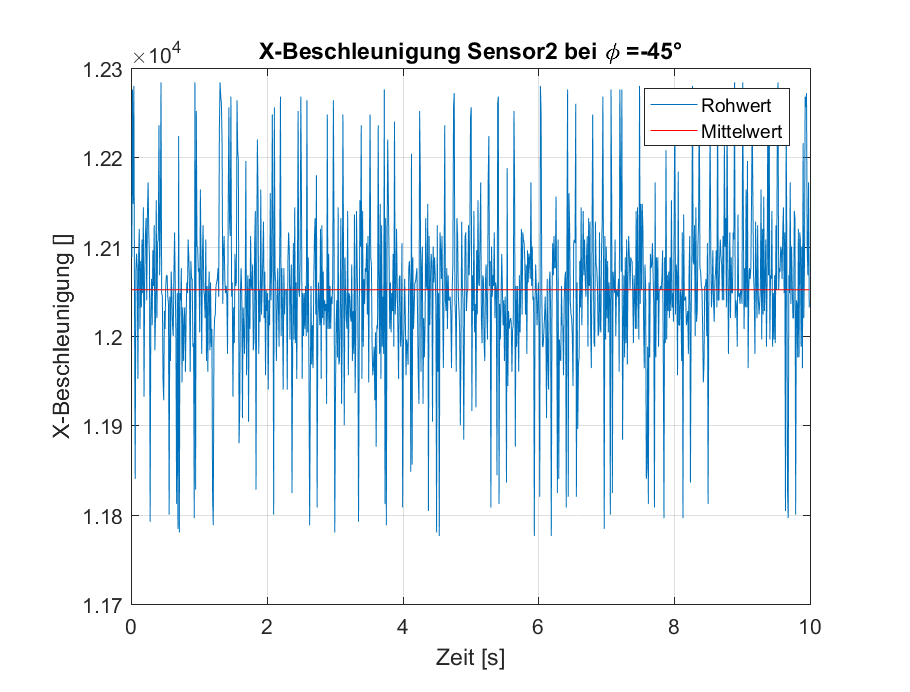
\includegraphics[width=0.5\linewidth]{img/X2__dd___phi_-45.eps}
\end{figure}
\begin{figure}[h]
	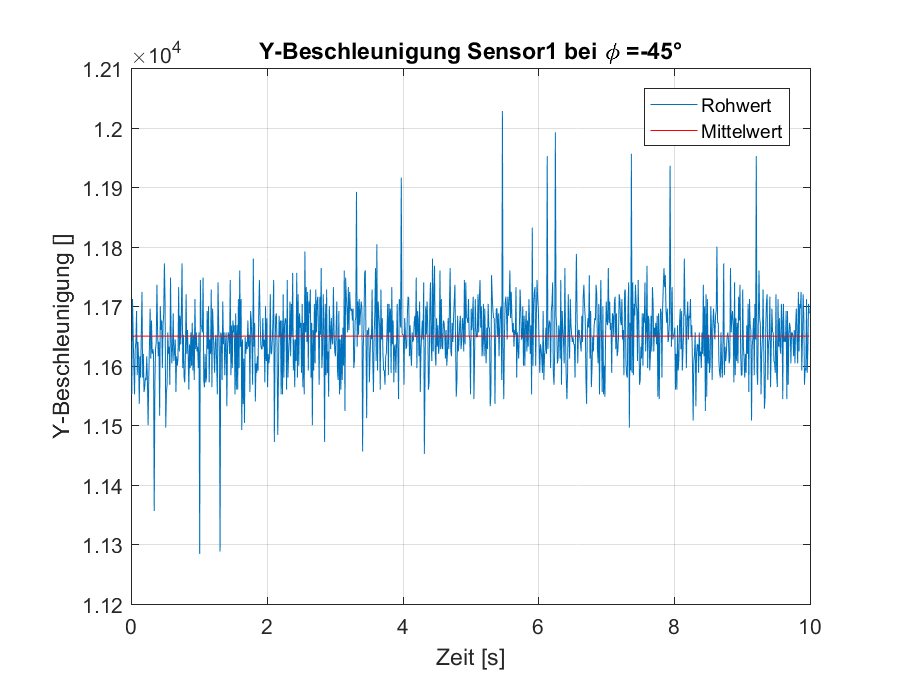
\includegraphics[width=0.5\linewidth]{img/Y1__dd___phi_-45.eps}
	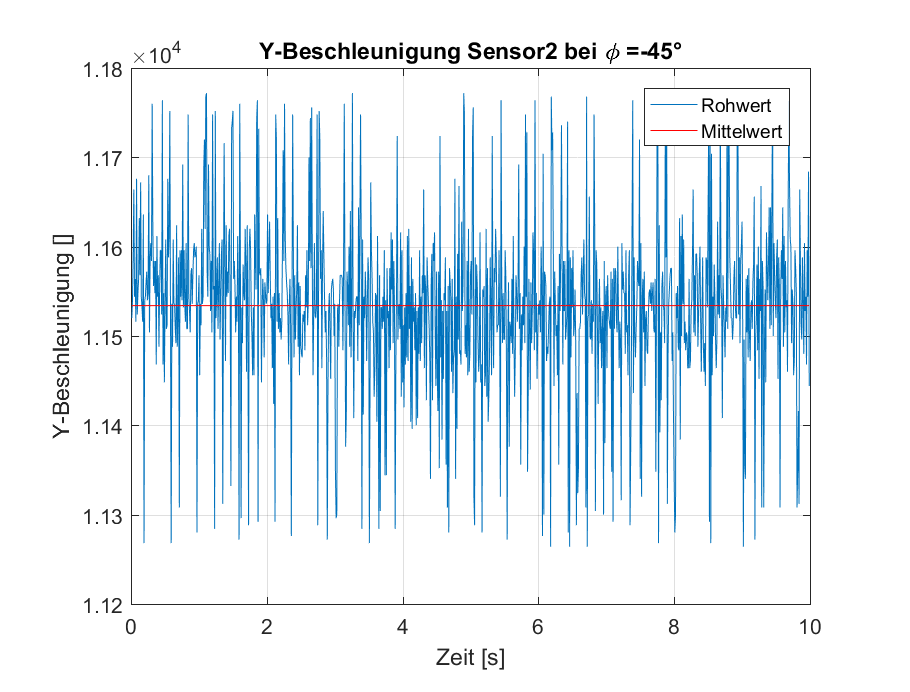
\includegraphics[width=0.5\linewidth]{img/Y2__dd___phi_-45.eps}
\end{figure}

\newpage
{\subsubsection{Rohwerte bei $\varphi = -30^{\circ}$}
\begin{figure}[h]
	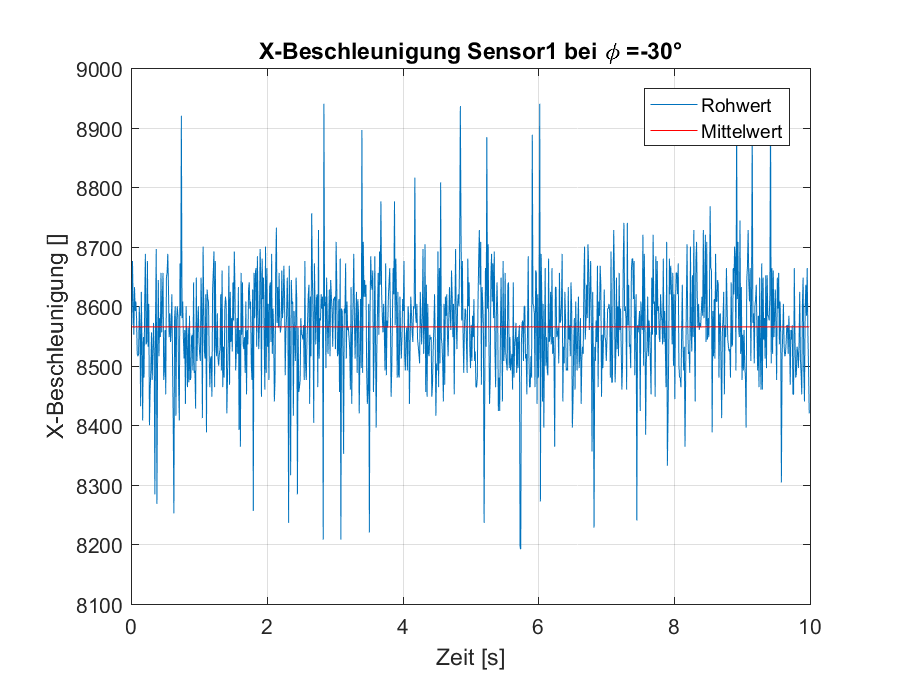
\includegraphics[width=0.5\linewidth]{img/X1__dd___phi_-30.eps}
	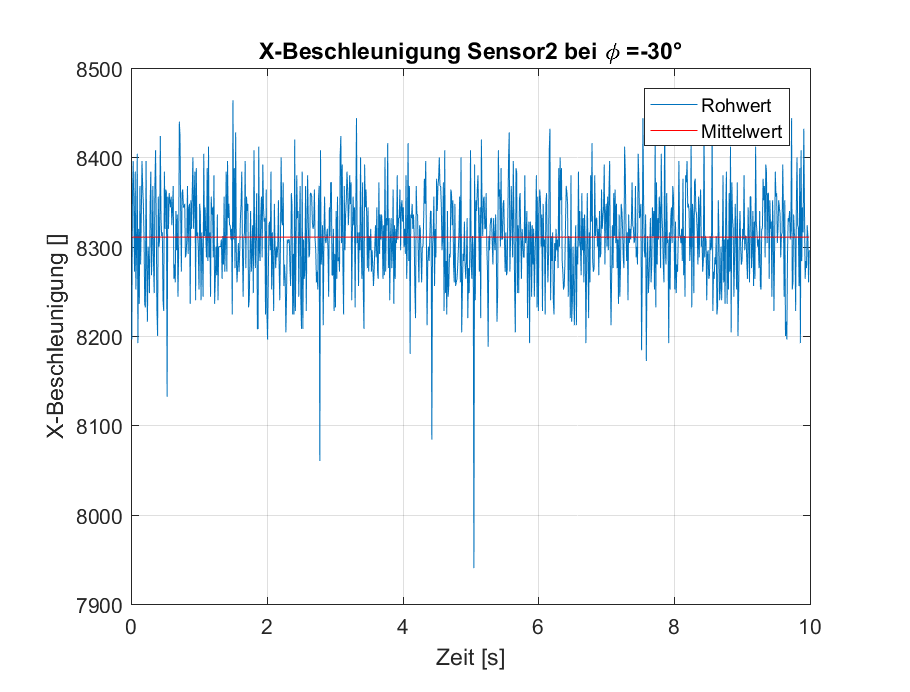
\includegraphics[width=0.5\linewidth]{img/X2__dd___phi_-30.eps}
\end{figure}
\begin{figure}[h]
	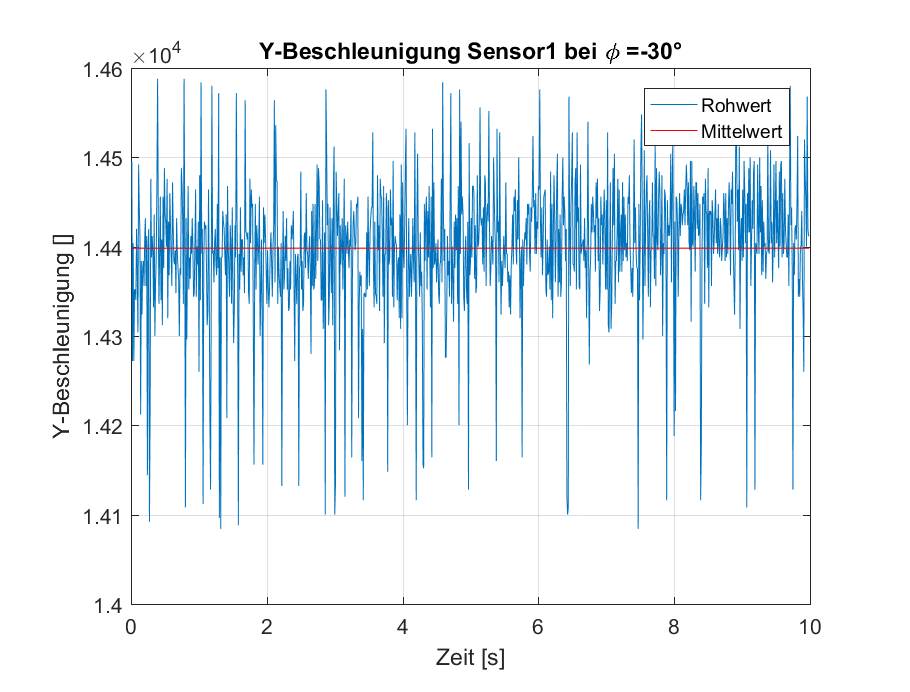
\includegraphics[width=0.5\linewidth]{img/Y1__dd___phi_-30.eps}
	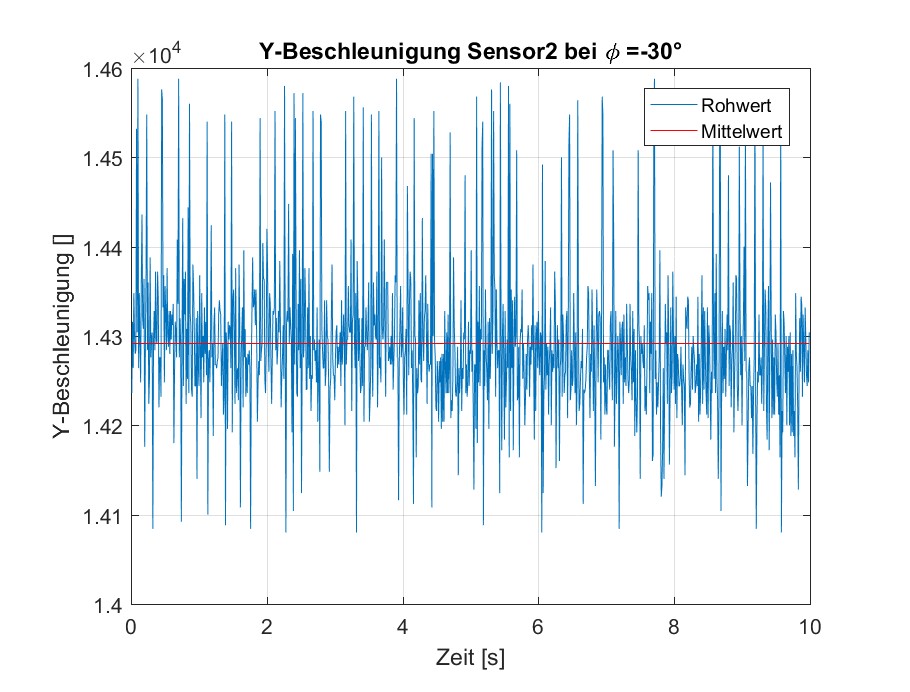
\includegraphics[width=0.5\linewidth]{img/Y2__dd___phi_-30.eps}
\end{figure}}

\newpage
{\subsubsection{Rohwerte bei $\varphi = -15^{\circ}$}
\begin{figure}[h]
	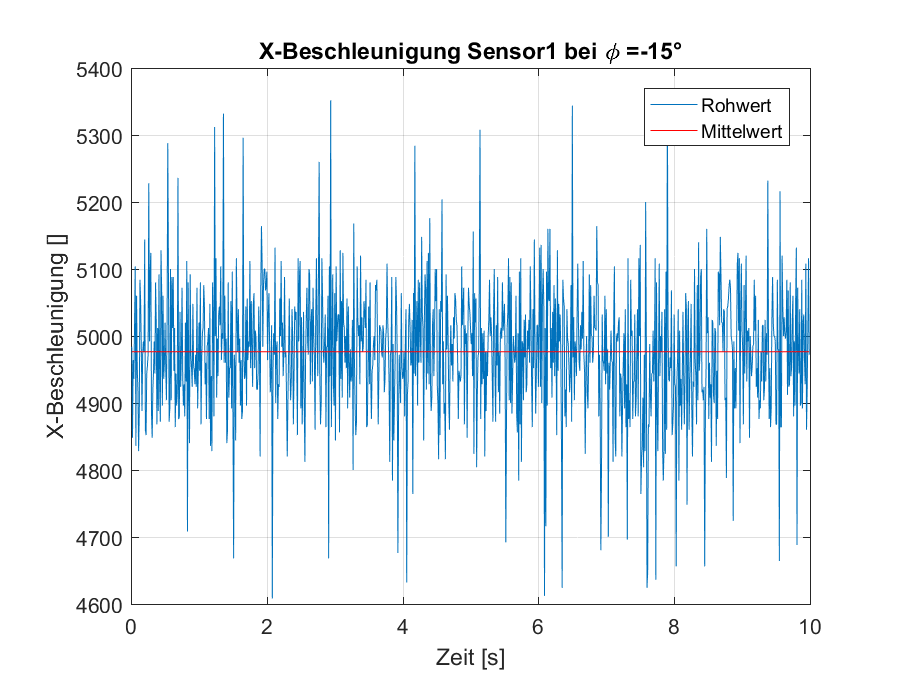
\includegraphics[width=0.5\linewidth]{img/X1__dd___phi_-15.eps}
	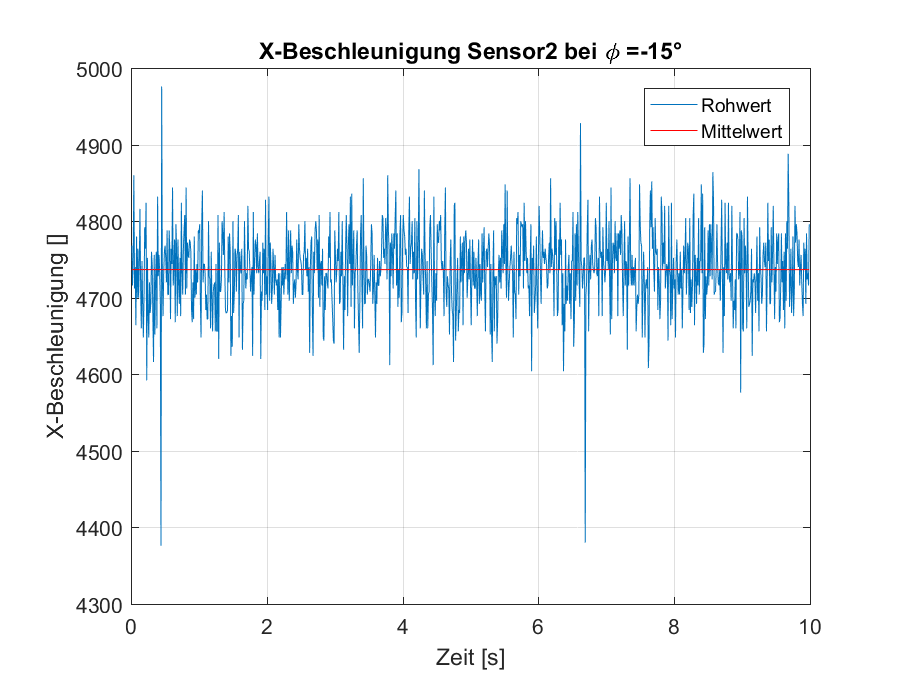
\includegraphics[width=0.5\linewidth]{img/X2__dd___phi_-15.eps}
\end{figure}
\begin{figure}[h]
	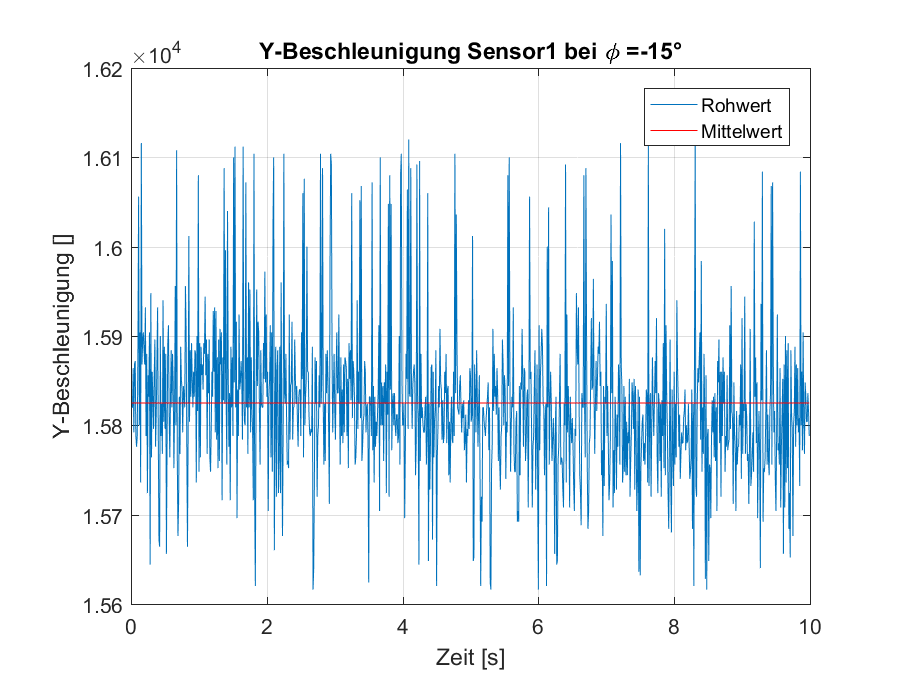
\includegraphics[width=0.5\linewidth]{img/Y1__dd___phi_-15.eps}
	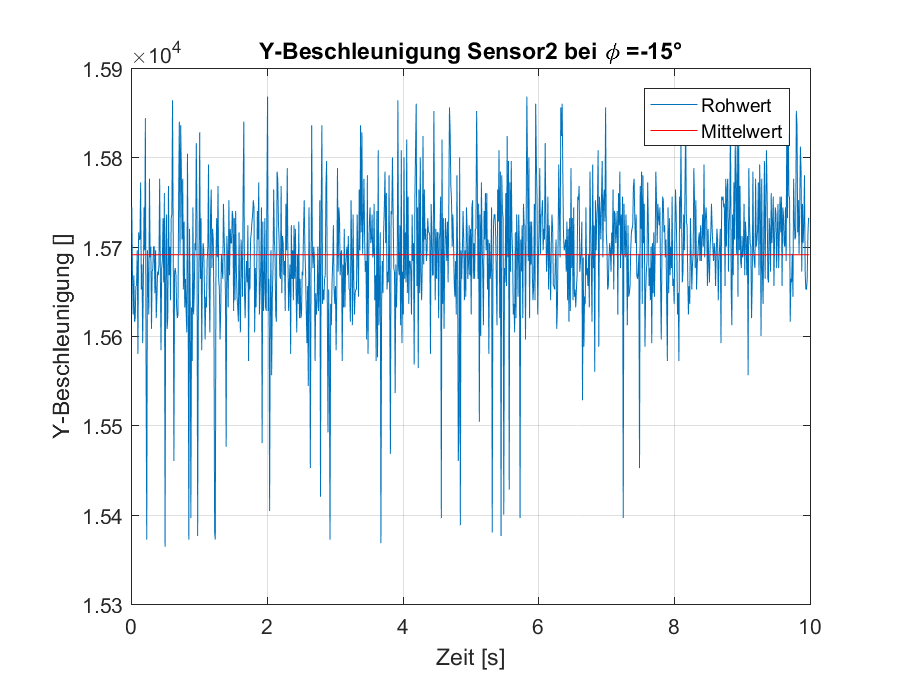
\includegraphics[width=0.5\linewidth]{img/Y2__dd___phi_-15.eps}
\end{figure}}

\newpage
{\subsubsection{Rohwerte bei $\varphi = 0^{\circ}$}
\begin{figure}[h]
	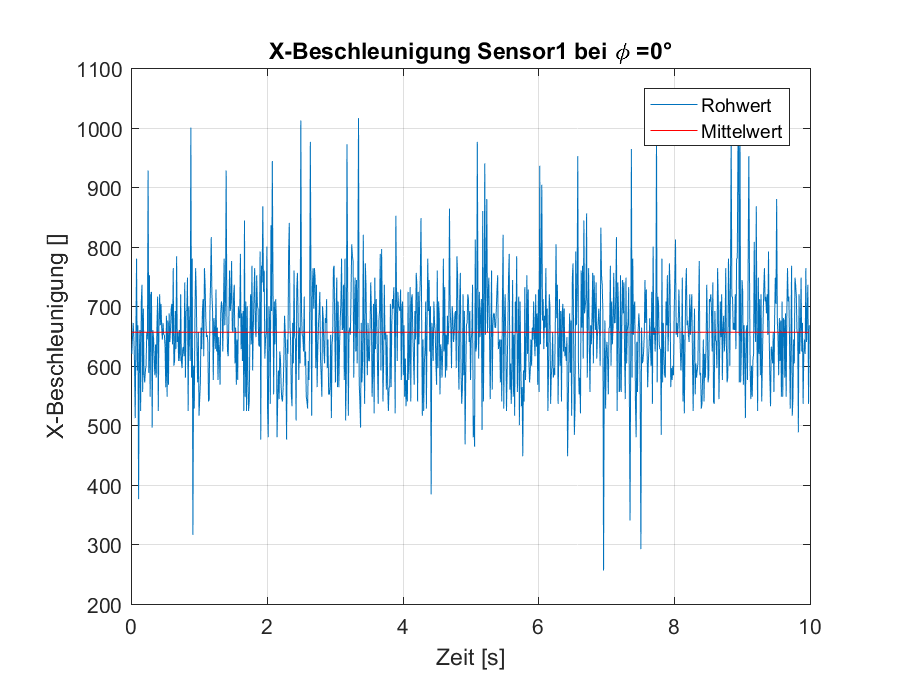
\includegraphics[width=0.5\linewidth]{img/X1__dd___phi_0.eps}
	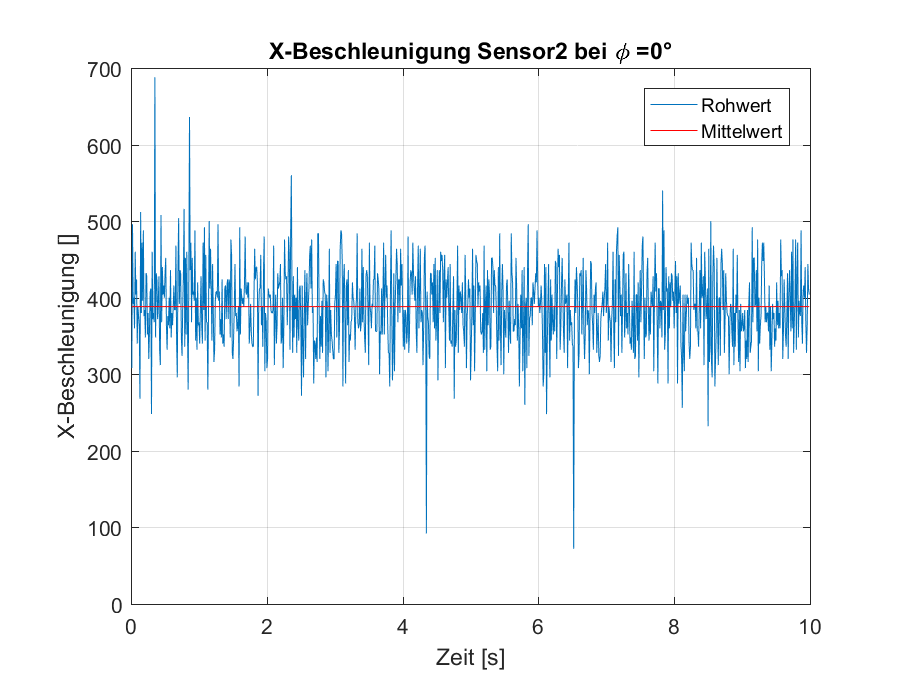
\includegraphics[width=0.5\linewidth]{img/X2__dd___phi_0.eps}
\end{figure}
\begin{figure}[h]
	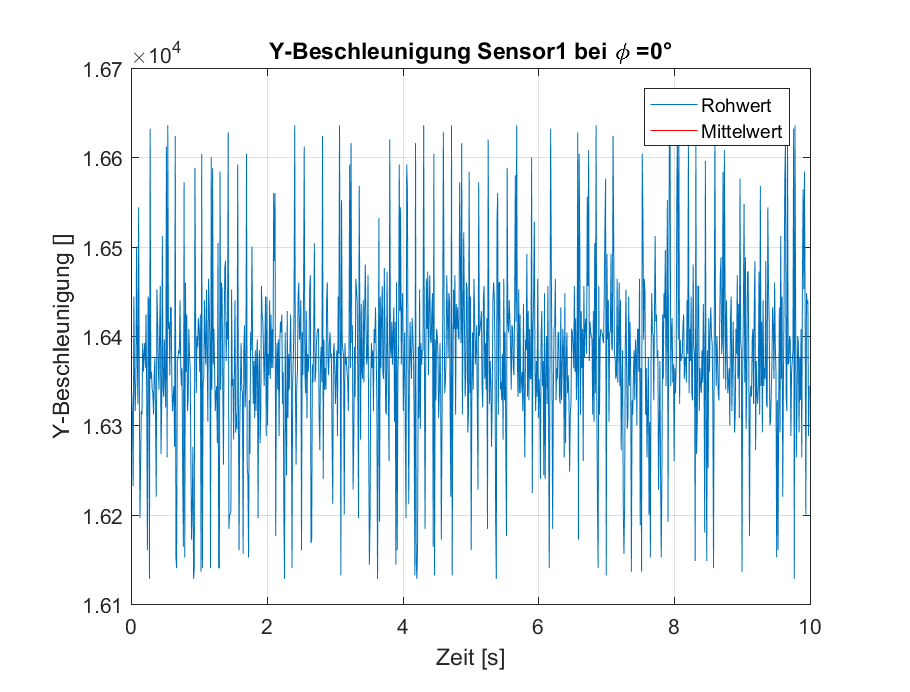
\includegraphics[width=0.5\linewidth]{img/Y1__dd___phi_0.eps}
	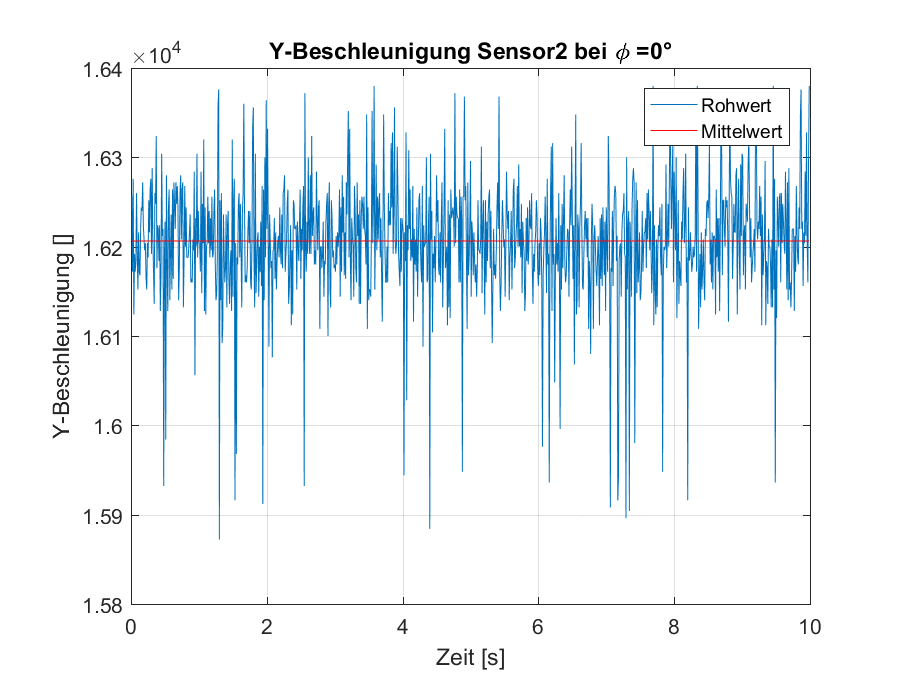
\includegraphics[width=0.5\linewidth]{img/Y2__dd___phi_0.eps}
\end{figure}}

\newpage
{\subsubsection{Rohwerte bei $\varphi = 15^{\circ}$}
\begin{figure}[h]
	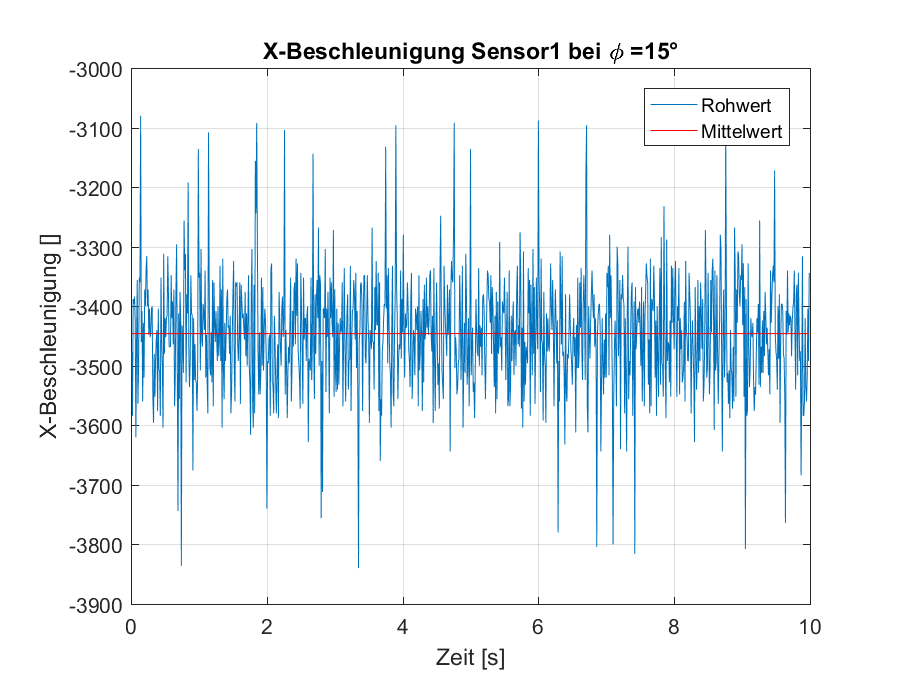
\includegraphics[width=0.5\linewidth]{img/X1__dd___phi_15.eps}
	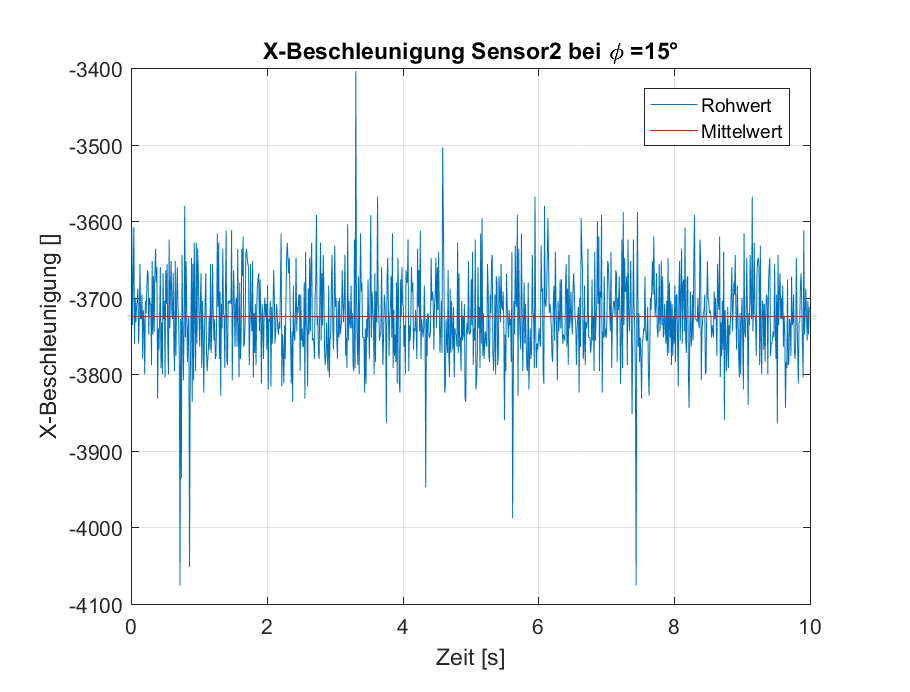
\includegraphics[width=0.5\linewidth]{img/X2__dd___phi_15.eps}
\end{figure}
\begin{figure}[h]
	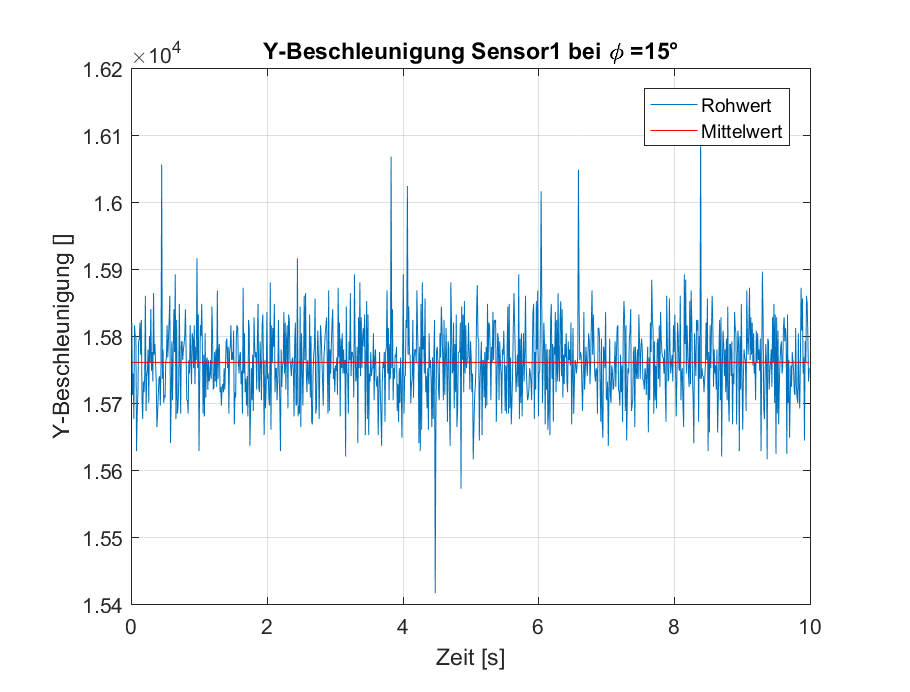
\includegraphics[width=0.5\linewidth]{img/Y1__dd___phi_15.eps}
	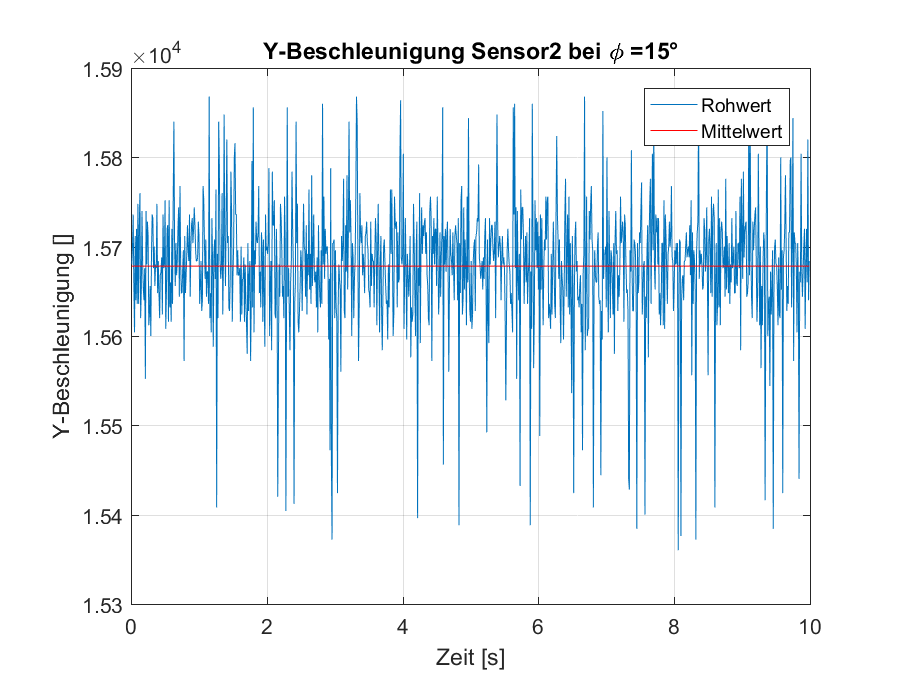
\includegraphics[width=0.5\linewidth]{img/Y2__dd___phi_15.eps}
\end{figure}}

\newpage
{\subsubsection{Rohwerte bei $\varphi = 30^{\circ}$}
\begin{figure}[h]
	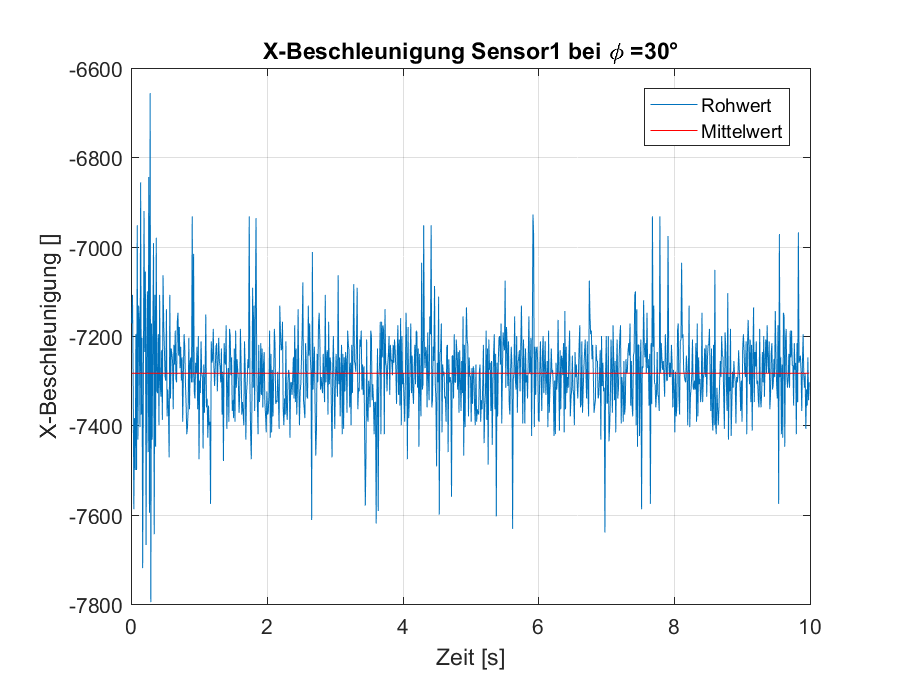
\includegraphics[width=0.5\linewidth]{img/X1__dd___phi_30.eps}
	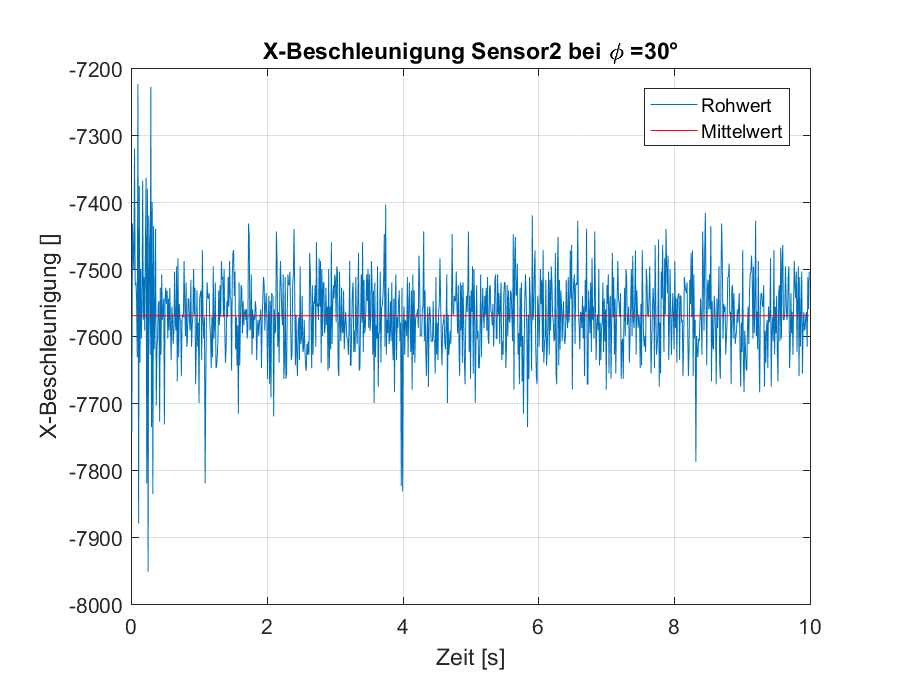
\includegraphics[width=0.5\linewidth]{img/X2__dd___phi_30.eps}
\end{figure}
\begin{figure}[h]
	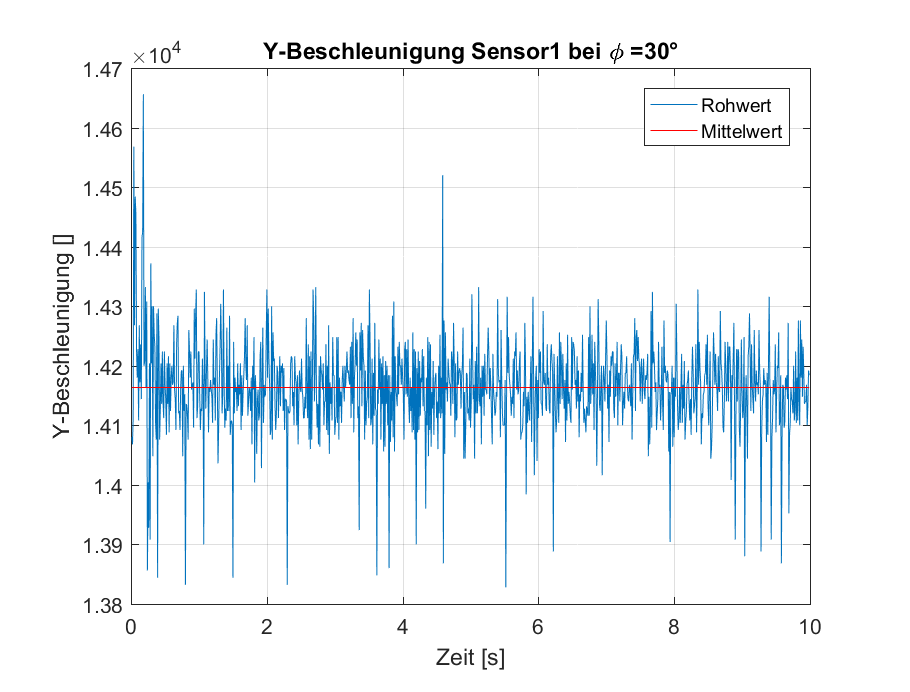
\includegraphics[width=0.5\linewidth]{img/Y1__dd___phi_30.eps}
	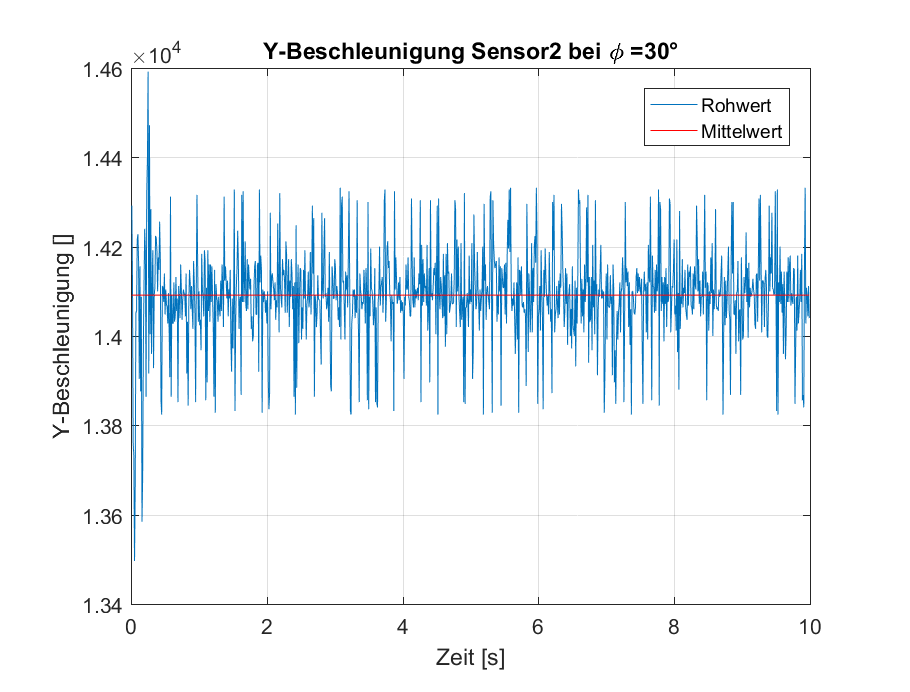
\includegraphics[width=0.5\linewidth]{img/Y2__dd___phi_30.eps}
\end{figure}}

\newpage
{\subsubsection{Rohwerte bei $\varphi = 45^{\circ}$}
\begin{figure}[h]
	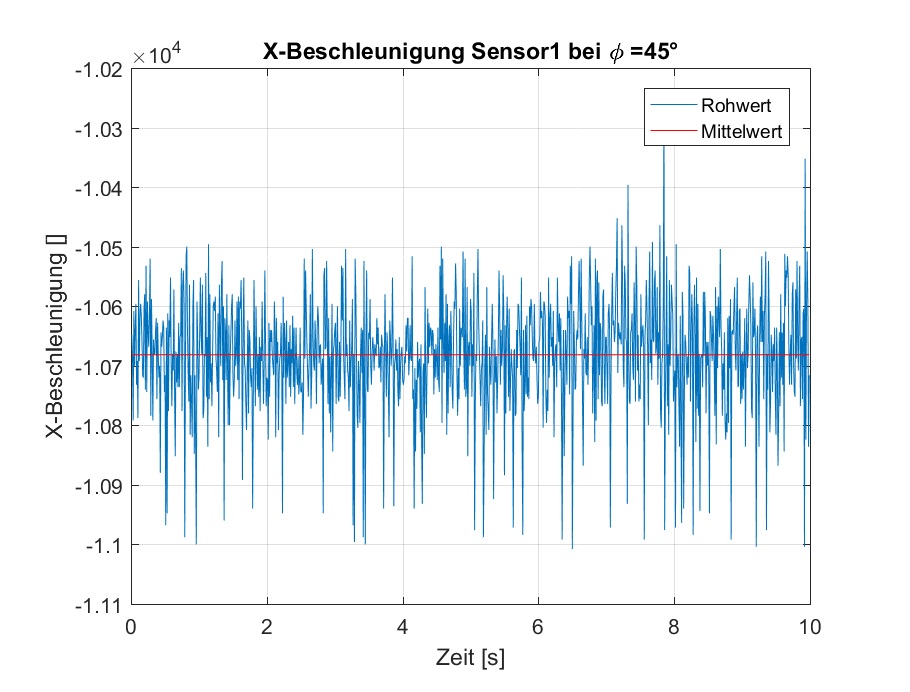
\includegraphics[width=0.5\linewidth]{img/X1__dd___phi_45.eps}
	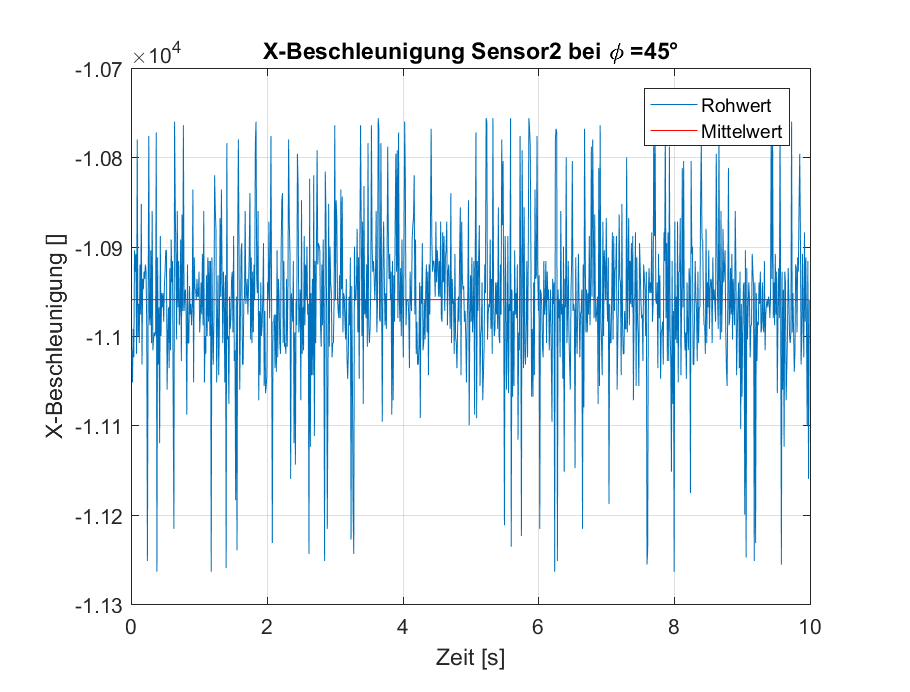
\includegraphics[width=0.5\linewidth]{img/X2__dd___phi_45.eps}
\end{figure}
\begin{figure}[h]
	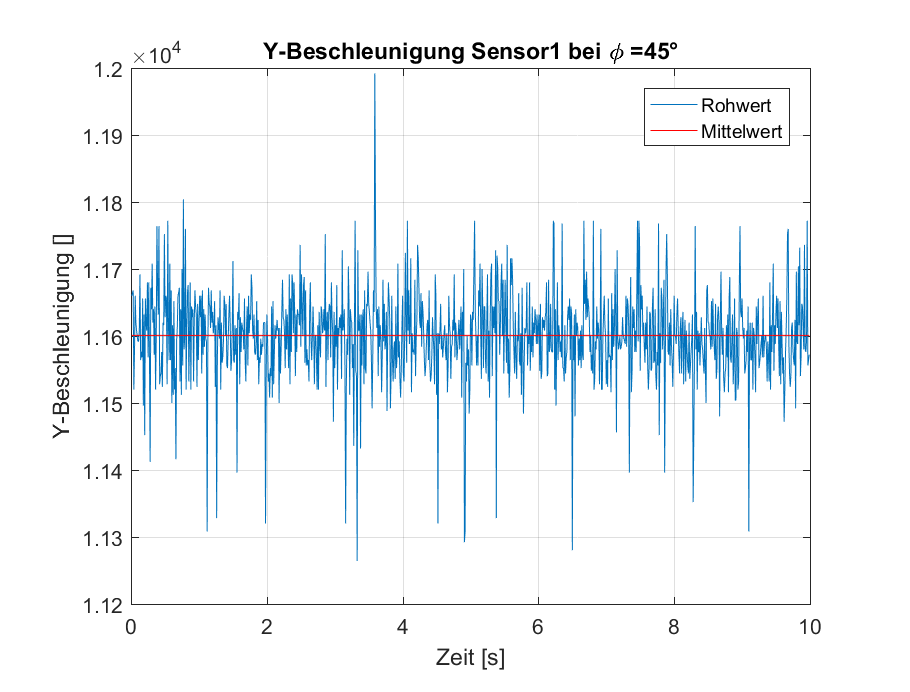
\includegraphics[width=0.5\linewidth]{img/Y1__dd___phi_45.eps}
	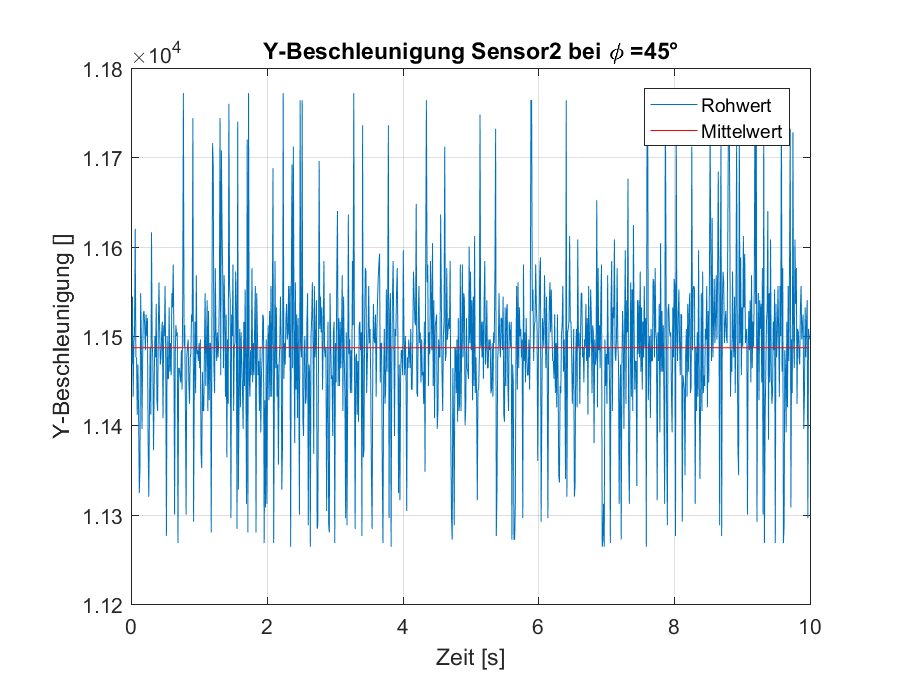
\includegraphics[width=0.5\linewidth]{img/Y2__dd___phi_45.eps}
\end{figure}}

\newpage
\subsection{Mittelwertverlauf und Ausgleichspolynom}
Für jede Achse der beiden Sensoren ergeben sich aus den obigen Aufzeichnungen ein Vektor, welcher den Verlauf der Mittelwerte beschreibt. Da die Sollbeschleunigung bekannt ist kann nun ein Polynom erster Ordnung bestimmt werden, welches die Rohdaten in Beschleunigungswerte umrechnet. Die folgenden Abbildungen zeigen den Verlauf der Sollwerte und die Ergebnisse der Umrechnung.


\begin{table}[h]
\centering
\begin{tabular}{lcllcl}
$\ddot{x}_n$ &$\equiv$& X-Beschleunigung Sensor n &
$\ddot{x}^R_n$ &$\equiv$& X-Rohwert Sensor n \\
$\ddot{y}_n$ &$\equiv$& Y-Beschleunigung Sensor n &
$\ddot{y}^R_n$ &$\equiv$& Y-Rohwert Sensor n
\end{tabular}
\end{table}

\vspace*{-\baselineskip}
\begin{equation}
\ddot{x}_n = p^1_{x_n} \cdot \ddot{x}^R_n + p^2_{x_n} \hspace{35pt} \vert \hspace{3pt} n \in \{1, 2\}
\end{equation}
\begin{equation}
\ddot{y}_n = p^1_{y_n} \cdot \ddot{y}^R_n + p^2_{y_n} \hspace{35pt} \vert \hspace{3pt} n \in \{1, 2\}
\end{equation}
\vspace*{-\baselineskip}
\begin{table}[h]
\centering
\begin{tabular}{lcllcl}
$p^1_{x_1}$ &$=$& $-6.082 \cdot 10^{-4}$ & $p^2_{x_1}$ &$=$& $0.4412$ \\
$p^1_{x_2}$ &$=$& $-6.07 \cdot 10^{-4}$ & $p^2_{x_2}$ &$=$& $0.2804$ \\
$p^1_{y_1}$ &$=$& $-6.064 \cdot 10^{-4}$ & $p^2_{y_1}$ &$=$& $0.1248$ \\
$p^1_{y_2}$ &$=$& $-6.089 \cdot 10^{-4}$ & $p^2_{y_2}$ &$=$& $0.09182$ \\
\end{tabular}
\end{table}

\vspace*{-\baselineskip}
\begin{figure}[h]
	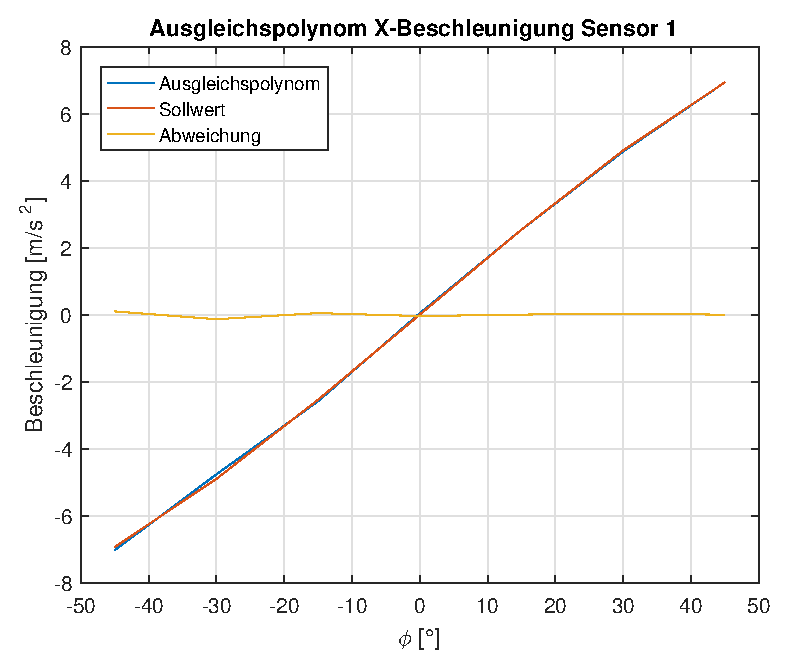
\includegraphics[width=0.5\linewidth]{img/X1__dd___fitted.eps}
	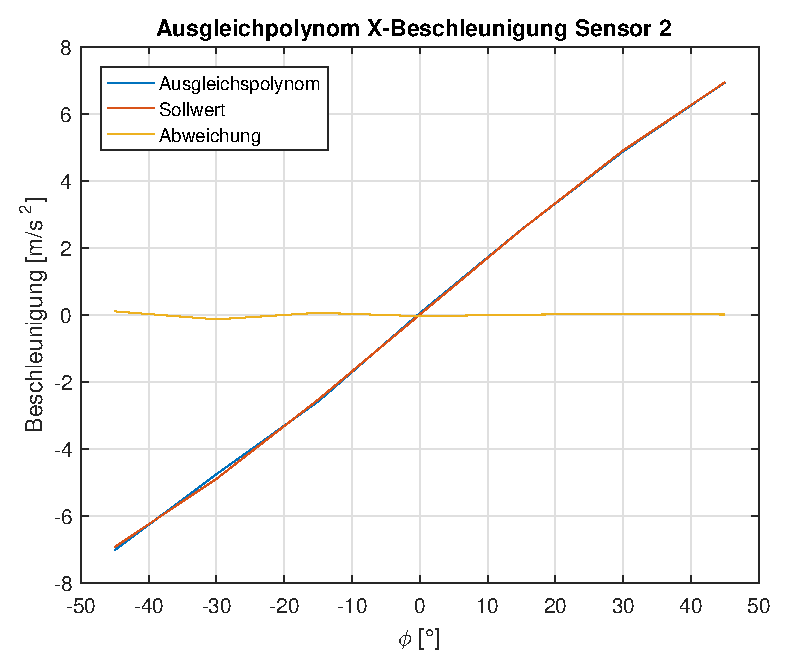
\includegraphics[width=0.5\linewidth]{img/X2__dd___fitted.eps}
\end{figure}

\vspace*{-\baselineskip}
\begin{figure}[h!]
	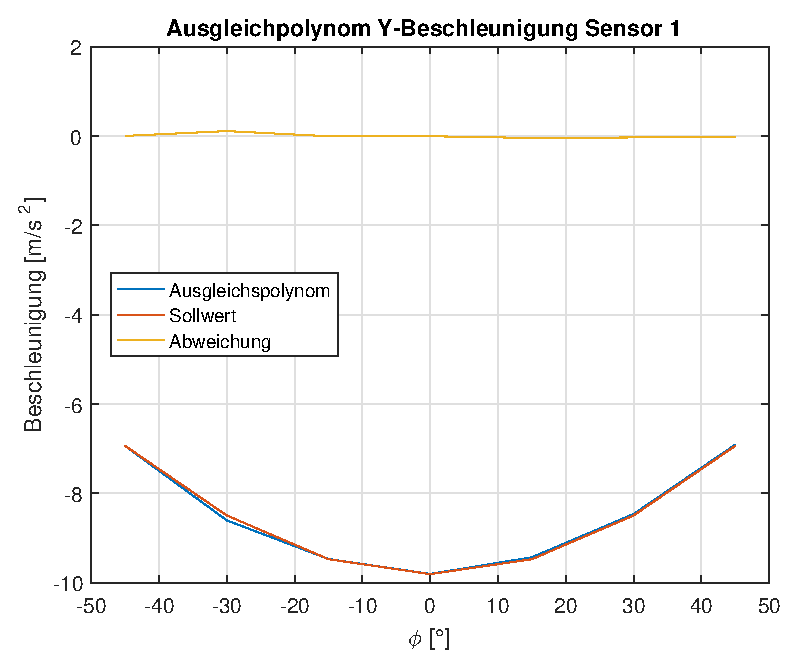
\includegraphics[width=0.5\linewidth]{img/Y1__dd___fitted.eps}
	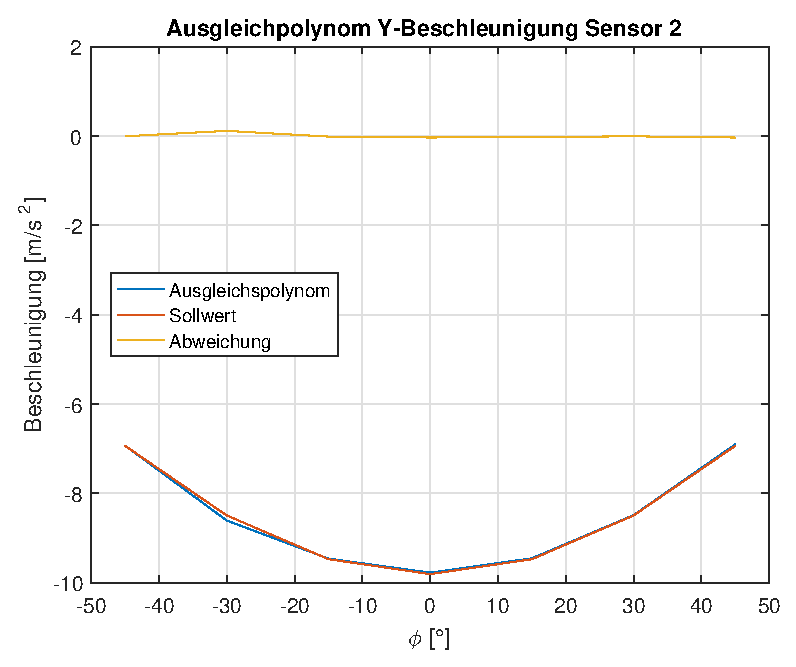
\includegraphics[width=0.5\linewidth]{img/Y2__dd___fitted.eps}
\end{figure}

